%----------------------------------------------------------------------------------------
%	PACKAGES AND DOCUMENT CONFIGURATIONS
%----------------------------------------------------------------------------------------

\documentclass[10pt,a4paper]{article}

% Adjusting margins
\addtolength{\oddsidemargin}{-.5in}
\addtolength{\evensidemargin}{-.5in}
\addtolength{\textwidth}{1in}
\addtolength{\topmargin}{-.5in}
\addtolength{\textheight}{1in}

% Graphics
\usepackage{caption}
\usepackage{subcaption}
\usepackage{graphicx}
\graphicspath{{figures/}}

% Math
\usepackage{amssymb}
\usepackage{amsmath}
\usepackage{amsthm}
\usepackage{mathtools}

% Theorems and proofs
\newtheorem{proposition}{Proposition}[section]
\newtheorem{definition}[proposition]{Definition}
\newtheorem{corollary}[proposition]{Corollary}
\theoremstyle{remark}
\newtheorem*{remark}{Remark}

% Other
\usepackage{algorithmic}
\usepackage{array}
\usepackage{booktabs}
\usepackage{hyperref}
\usepackage[english]{babel}
\usepackage{enumitem}
\usepackage{xcolor}

% ---- Additions over the BXINT4 template preamble (three only) --------------
% Times-compatible text and math: the body font must match the Times-like
% serif used inside the generated figures, so figure labels and captions do
% not visibly change typeface at the figure boundary.
\usepackage{newtxtext,newtxmath}
% SI units: capacities are reported in GiB and rates in requests per second,
% so unit macros avoid hand-written and inconsistent unit strings.
\usepackage{siunitx}
% Cross-references: every reference must name its own type (Section, Table,
% Figure, Equation) to keep the long appendix readable. Loaded after hyperref.
\usepackage{cleveref}
% ---------------------------------------------------------------------------

\hypersetup{
    colorlinks=true,
    linkcolor=blue,
    citecolor=blue,
    urlcolor=blue
}

%----------------------------------------------------------------------------------------
%	PAGE BUDGET (binding, checked before submission)
%----------------------------------------------------------------------------------------
% Main body, Section 1 through Section 6: 8 to 10 pages.
% References: 1 page, not counted against the body budget.
% Appendix: unlimited, ordered derivations, hyperparameters, per-cluster
%   numbers, reproducibility commands.
% Enforcement: the body is assembled only from sections/01 through
%   sections/06. Any material that pushes the body past 10 pages moves to
%   sections/appendix.tex rather than compressing the argument.
% The anchor for this budget is \label{sec:pagebudget} in Section 1.
%----------------------------------------------------------------------------------------


%----------------------------------------------------------------------------------------
%	MAIN PART
%----------------------------------------------------------------------------------------
\begin{document}

\title{Cache Hit-Ratio Curves from Reuse Distance: A Survival Model on Production Traces}
\author{Syed Ibrahim Omer}
\date{\today}
\maketitle


%----------------------------------------------------------------------------------------
%	Abstract
%----------------------------------------------------------------------------------------
\begin{abstract}
\noindent
Miss-ratio curves (MRCs) report the hit ratio of a cache as a function of its
capacity, and they drive memory provisioning decisions in production cache
fleets. Current practice fits the aggregate hit count, or the aggregate miss
ratio, as a function of capacity, which discards the per-request structure that
determines where a curve bends. We instead treat the reuse distance of each
request as a positive integer survival time and estimate its discrete hazard
with gradient-boosted decision trees. The resulting survival function maps
directly onto the MRC through the LRU stack property, so capacity is a
post-hoc evaluation point rather than a regressor input.

The report formalizes reuse distance as a censored discrete time-to-event
variable, states the identification condition that ties it to LRU hit behavior,
and specifies two gradient-boosted hazard parametrizations: reuse distance as a
feature, and one model per hazard bin. Censoring is handled explicitly, because
requests whose reuse distance exceeds the observation window are not misses at
a known distance but unresolved observations. Evaluation is against MRCs
obtained from full trace simulation on production clusters, using MRC error,
hazard calibration, and the integrated Brier score. All quantitative results in
this skeleton are placeholders; no numbers are reported until the simulation
and model runs complete.
\end{abstract}


%----------------------------------------------------------------------------------------
%	Table of Contents
%----------------------------------------------------------------------------------------
\setcounter{tocdepth}{2}
\tableofcontents

\clearpage

%----------------------------------------------------------------------------------------
%	Main Part
%----------------------------------------------------------------------------------------
\section{Introduction}
\label{sec:introduction}

A miss-ratio curve (MRC) gives the hit ratio $H(C)$ of a cache of capacity $C$
on a given request stream. Operators use it to size memory: the capacity at
which the curve flattens is the point past which additional memory buys little
hit ratio. Published fleet analyses show that capacity decisions of this kind
are made continuously across hundreds of clusters \cite{yang2020}.

\subsection{The Gap: Aggregate Regression}

The dominant practical approach regresses an aggregate hit count, or an
aggregate miss ratio, on capacity. The fit is performed over a set of measured
capacities, and the curve is interpolated or extrapolated from those points.
This formulation has two costs. First, capacity enters as a covariate, so every
new capacity requires new measurements or a new fit. Second, aggregating over
requests removes the per-request quantity that actually governs the curve: how
far back in the stream a request must reach to find its previous access. Two
workloads with identical aggregate hit counts at one capacity can have
different curves at every other capacity, and aggregate regression cannot
distinguish them.

\subsection{Motivation: Over- and Under-Allocation}

Both directions of sizing error are expensive. Over-allocation reserves memory
that produces no hit-ratio gain, which in a multi-tenant fleet is memory taken
from another workload. Under-allocation produces misses that fall through to
the storage tier, where the latency penalty is orders of magnitude larger than
a cache lookup. A curve that is accurate in shape, and not only at the
capacities that were measured, supports sizing at capacities that were never
observed. That is the operational motivation for modelling the per-request
reuse process instead of its aggregate.

\subsection{Contributions}

\begin{enumerate}[nosep]
    \item A formulation of reuse distance as a right-censored discrete
    time-to-event variable, with the LRU stack property supplying the exact map
    from its survival function to the MRC (Section~\ref{sec:formalization}).
    \item Two gradient-boosted discrete hazard parametrizations, one treating
    reuse distance as a feature and one fitting a separate model per hazard
    bin, together with an explicit censoring correction and a documented
    Optuna search space (Section~\ref{sec:methods}).
    \item An evaluation protocol against simulation ground truth on production
    traces, reporting MRC error, hazard calibration, and the integrated Brier
    score rather than a single aggregate fit statistic
    (Section~\ref{sec:experiments}).
\end{enumerate}

\subsection*{Scope and Page Budget}
\phantomsection\label{sec:pagebudget}

% PAGE BUDGET: body 8-10 pages (Sections 1-6). References and appendix are
% outside the budget. Derivations, full hyperparameter tables, per-cluster
% numbers and reproduction commands live in the appendix by design, so that
% the body states the argument and the appendix carries the evidence.
The body of this report is budgeted at eight to ten pages, following the
allocation recorded in \texttt{main.tex} and anchored at
Section~\ref{sec:pagebudget}. Material that does not fit moves to the appendix
rather than being compressed. The report covers LRU-referenced MRCs only;
non-LRU replacement is discussed as a limitation in
Section~\ref{sec:conclusion}.

\section{Related Work}
\label{sec:related-work}

\subsection{Stack Distance and Reuse Distance}

Mattson et al.\ introduced the stack algorithm and the distance between
successive references to a block, and proved that LRU hit behavior at capacity
$C$ is determined by counting distinct blocks referenced since the previous
access \cite{mattson1970}. Hill and Smith developed the miss-ratio curve as a
first-class object, computing all-miss-ratio curves by simulating a set of
capacities and showing how curve shape distinguishes compulsory, capacity and
conflict misses \cite{hill1989}. Both results are exact for the reference
stream they are computed on; neither is a statistical model, and neither
extrapolates to unobserved capacities.

\subsection{Approximate MRC Construction}

Exact stack distance computation costs time linear in the trace length times
the number of distinct blocks. Counter stacks replace per-reference search with
a compact data structure that yields stack distance histograms for many
capacities in one pass \cite{wires2014}. SHARDS obtains MRCs at scale by
sampling references into miniature simulations, correcting the resulting
downsampling bias analytically, and aggregating per-simulation histograms
\cite{waldspurger2015}. These methods are the ground truth against which a
model is judged here: simulation is accurate up to sampling error, and its cost
is what a model is meant to avoid on every capacity query.

\subsection{Reuse-Distance Analysis}

Reuse distance analysis extends the single-parameter stack model to arbitrary
replacement policies by tracking the reuse distance of each request and
replaying it against a policy-specific recency structure
\cite{beckmann2016,beckmann2017}. This line of work establishes that reuse
distance is a sufficient statistic for a broad class of policies, which is the
premise the present model relies on for LRU and only for LRU. Production trace
studies supply the workload evidence: the Twitter cache analysis reports
reuse-distance and miss-ratio structure across hundreds of in-memory clusters
and motivates cluster-level heterogeneity as a modelling concern
\cite{yang2020}.

\subsection{Survival Analysis in Systems Contexts}

Reuse distance is a positive, integer-valued waiting time, observed under a
truncation that depends on the observation window. That is a censored
time-to-event problem, and the discrete hazard formulation used here follows
the Kaplan-Meier product-limit estimator for right-censored data
\cite{kaplan1958} and the proportional hazards regression of Cox
\cite{cox1972}. Grouped and interval-censored observations, which arise when
reuse distance is binned, are treated by the Turnbull estimator
\cite{turnbull1976}. Gradient boosting supplies the flexible hazard component:
gradient-boosted decision trees \cite{friedman2001} as implemented in LightGBM
\cite{ke2017}, with hyperparameters selected by Optuna \cite{akiba2019}. The
combination of a nonparametric hazard with a tree ensemble is standard in
survival regression; the contribution here is the mapping of that hazard onto
cache capacity rather than onto a clinical or reliability endpoint.

\section{Formalization}
\label{sec:formalization}

\captionsetup{hypcap=false}

A miss-ratio curve is the survival function of the backward reuse distance,
parametrized by a discrete hazard on a log-spaced bin grid. This section states the
one censoring mechanism and the capacity range it identifies, and fixes the
metrics.

\subsection{Backward Reuse Distance}

For request $i$ with key $k_i$, let $p(i) = \max\{j < i : k_j = k_i\}$ be the
position of the previous access to the same key, and $p(i) = \bot$ when the key has
not been requested earlier in the window. The reuse distance is the number of
distinct keys requested strictly between the two accesses,
\begin{equation}\label{eq:reuse}
    R_i \;=\; \bigl|\{\, k_j : p(i) < j < i \,\}\bigr|,
\end{equation}
with $R_i = \infty$ when $p(i) = \bot$.

\begin{center}
\begin{minipage}{\linewidth}
\footnotesize
\captionof{table}{Symbols of \cref{eq:reuse}.}
\label{tab:sym-reuse}
\begin{tabular}{@{}l l l@{}}
\toprule
Symbol & Domain & Meaning and units \\
\midrule
$i, j$ & $\{1,\dots,N\}$ & request index in the window (count) \\
$k_i$ & $\mathcal{K}$ & key of request $i$ (identifier) \\
$p(i)$ & $\{1,\dots,N\} \cup \{\bot\}$ & previous access to $k_i$ (request index) \\
$R_i$ & $\mathbb{N}_0 \cup \{\infty\}$ & backward reuse distance (distinct keys, equivalently objects) \\
\bottomrule
\end{tabular}
\end{minipage}
\end{center}

A backward distance depends on the past only, so it is observed for every request
whose previous access lies inside the window, and the window end does not censor it.

\subsection{Miss Ratio as a Survival Function}

\begin{proposition}[LRU hit condition]\label{prop:lru-hit}
Under LRU replacement with capacity $C$ objects, a repeated request $i$ hits if and
only if $R_i < C$.
\end{proposition}

\begin{proof}
Before request $i$ the cache holds the $C$ most recently requested distinct keys.
The keys requested after $p(i)$ are exactly the keys more recent than $k_i$, and
they are distinct, so they occupy $R_i$ recency positions above $k_i$. The key
$k_i$ is resident if and only if $R_i < C$, the stack property established by
Mattson et al.~\cite{mattson1970}.
\end{proof}

Write $B = \mathrm{bin}(R)$ for the bin index of the reuse distance and $X$ for the
feature vector of a request. The miss ratio at capacity $C$ is the probability that
a repeated request misses, averaged over requests, plus the compulsory mass that no
capacity can recover:
\begin{equation}\label{eq:mrc}
    m(C) \;=\; p_c \;+\; (1 - p_c)\,\frac{1}{N}\sum_{i=1}^{N} S_{k(C)}(x_i),
    \qquad k(C) = \mathrm{bin}(C - 1),
\end{equation}
with $S_k(x) = \Pr(R \ge b_{k+1} \mid X = x)$ the survival through bin $k$ and
$b_{k+1}$ that bin's upper edge.

\begin{center}
\begin{minipage}{\linewidth}
\footnotesize
\captionof{table}{Symbols of \cref{eq:mrc}.}
\label{tab:sym-mrc}
\begin{tabular}{@{}l l l@{}}
\toprule
Symbol & Domain & Meaning and units \\
\midrule
$C$ & $\mathbb{N}$ & cache capacity (objects) \\
$m(C)$ & $[0,1]$ & miss ratio at capacity $C$ (dimensionless) \\
$p_c$ & $[0,1]$ & fraction of requests with no previous access in the window (dimensionless) \\
$N$ & $\mathbb{N}$ & requests in the scored block (count) \\
$x_i$ & $\mathbb{R}^{12}$ & feature vector of request $i$ (\cref{tab:features}) \\
$k(C)$ & $\{0,\dots,M-2\}$ & bin index of the largest distance below capacity $C$ (dimensionless) \\
$S_k(x)$ & $[0,1]$ & survival through bin $k$ (dimensionless) \\
$b_k$ & $\mathbb{N}_0$ & lower edge of bin $k$ (objects) \\
\bottomrule
\end{tabular}
\end{minipage}
\end{center}

\subsection{Discrete Hazard on Log-Spaced Bins}

The hazard of bin $b$ is the probability that the distance resolves in that bin
given that it reached the bin's lower edge, and survival multiplies the
non-resolution probabilities:

\begin{align}
    h_b(x) &= \Pr\bigl(B = b \mid B \ge b,\; X = x\bigr),
    \qquad b = 0, \dots, M-1, \label{eq:hazard}\\
    S_k(x) &= \prod_{b=0}^{k}\bigl(1 - h_b(x)\bigr),
    \qquad S_{-1}(x) = 1. \label{eq:survival}
\end{align}
The interior edges are a rounded geometric sequence over the observed 99.9th
percentile: $b_0 = 0$, $b_1 = 1$, and $b_2,\dots,b_M$ are the unique values of
$\operatorname{round}(2\gamma^{t})$ for $t = 0,\dots,M-1$, with
$\gamma = (\max(3,q)/2)^{1/(M-1)}$.

\begin{center}
\begin{minipage}{\linewidth}
\footnotesize
\captionof{table}{Symbols of \cref{eq:hazard}, \cref{eq:survival} and the edge sequence.}
\label{tab:sym-hazard}
\begin{tabular}{@{}l l l@{}}
\toprule
Symbol & Domain & Meaning and units \\
\midrule
$b$ & $\{0,\dots,M-1\}$ & bin index (dimensionless) \\
$B$ & $\{0,\dots,M-1\}$ & bin index of the observed reuse distance (dimensionless) \\
$h_b(x)$ & $[0,1]$ & discrete hazard of bin $b$ for features $x$ (dimensionless) \\
$S_k(x)$ & $[0,1]$ & survival through bins $0,\dots,k$ (dimensionless) \\
$M$ & $\mathbb{N}$ & requested number of bins (count) \\
$q$ & $\mathbb{N}$ & 99.9th percentile of $R$ over eligible requests (objects) \\
$\gamma$ & $\mathbb{R}_{>1}$ & geometric growth factor between interior edges (dimensionless) \\
$t$ & $\{0,\dots,M-1\}$ & index of the geometric sequence (dimensionless) \\
\bottomrule
\end{tabular}
\end{minipage}
\end{center}

Rounding collapses duplicates, so the realised bin count is reported: with $M=32$
requested the traces of \cref{sec:experiments} realise 33, 33 and 14 bins, the last
because its 99.9th percentile distance is 14 objects. Since the hazard is constant
within a bin, the capacity grid sits at interior bin upper edges, where
$S_{k(C)}$ and $\Pr(R \ge C)$ are the same event.

\subsection{The Only Censoring: the Observation Ceiling}

Two integers are retained per request, a truncated distance and an event indicator,
and the capacity grid is truncated at the same ceiling:
\begin{align}
    \tilde R_i &= \min(R_i,\, c), \qquad
    \delta_i = \mathbf{1}\{R_i \le c\}, \qquad c = b_{M-1} - 1,
    \label{eq:truncation}\\
    \mathcal{C} &\subset \{1, \dots, b_{M-1} - 1\}. \label{eq:limit}
\end{align}

\begin{center}
\begin{minipage}{\linewidth}
\footnotesize
\captionof{table}{Symbols of \cref{eq:truncation} and \cref{eq:limit}.}
\label{tab:sym-truncation}
\begin{tabular}{@{}l l l@{}}
\toprule
Symbol & Domain & Meaning and units \\
\midrule
$\tilde R_i$ & $\{0,\dots,c\}$ & truncated reuse distance (objects) \\
$\delta_i$ & $\{0,1\}$ & event indicator, zero when $R_i$ exceeds the cap (dimensionless) \\
$c$ & $\mathbb{N}_0$ & truncation cap, one object below the overflow edge (objects) \\
$\mathcal{C}$ & $2^{\mathbb{N}}$ & capacity grid, at most 24 points (objects) \\
$b_{M-1}$ & $\mathbb{N}$ & lower edge of the overflow bin (objects) \\
\bottomrule
\end{tabular}
\end{minipage}
\end{center}

The only censoring is administrative: distances at or above $b_{M-1}$ are pooled
into the overflow bin, so such a request is known only to have reached it,
contributes one row per lower bin labelled zero, and no positive label. A request
with no previous access inside the window leaves the fit and enters $p_c$, and some
of those are not compulsory in the workload's history, only in the window. The truth
uses the same convention, so the comparison is exact but conditional on a warm
start.

Survival above $b_{M-1}$ is not identified and the estimator refuses a capacity
there rather than extrapolating. The ceiling is 1{,}110{,}405, 37{,}455 and 13 objects
on the three traces of \cref{sec:experiments}, so the third is evaluated on 12
capacities of at most 12 objects.

\subsection{Metrics}

Let $\hat m$ be the estimated curve, $m$ the exact curve on the same block, and
$e(C) = \hat m(C) - m(C)$ the signed error at capacity $C$. On a grid
$\mathcal{C}$ of $n$ capacities the reported metrics are
\begin{align}
    \mathrm{MAE} &= \frac{1}{n}\sum_{C \in \mathcal{C}} \lvert e(C) \rvert, &
    \mathrm{MAX} &= \max_{C \in \mathcal{C}} \lvert e(C) \rvert, \label{eq:metrics-abs}\\
    \mathrm{bias} &= \frac{1}{n}\sum_{C \in \mathcal{C}} e(C), &
    \mathrm{MRE} &= \frac{1}{n_+}\sum_{C \in \mathcal{C}_+} \frac{\lvert e(C) \rvert}{m(C)},
    \label{eq:metrics-rel}\\
    \mathrm{ABC} &= \frac{1}{\log C_n - \log C_1}
    \int_{\log C_1}^{\log C_n} \lvert e(C) \rvert \; d\log C, & &
    \label{eq:abc}
\end{align}
where $\mathcal{C}_+ = \{C \in \mathcal{C} : m(C) \ge 0.01\}$ and $n_+ =
\lvert \mathcal{C}_+ \rvert$.

\begin{center}
\begin{minipage}{\linewidth}
\footnotesize
\captionof{table}{Symbols of \cref{eq:metrics-abs}, \cref{eq:metrics-rel} and \cref{eq:abc}.}
\label{tab:sym-metrics}
\begin{tabular}{@{}l l l@{}}
\toprule
Symbol & Domain & Meaning and units \\
\midrule
$\mathcal{C}$ & $2^{\mathbb{N}}$ & capacity grid, $\lvert\mathcal{C}\rvert = n$ (objects) \\
$n$ & $\mathbb{N}$ & number of grid points (count) \\
$C$ & $\mathbb{N}$ & one grid capacity (objects) \\
$\hat m(C)$ & $[0,1]$ & estimated miss ratio (dimensionless) \\
$m(C)$ & $[0,1]$ & exact miss ratio, $m(C) = \Pr(R \ge C)$ (dimensionless) \\
$e(C)$ & $[-1,1]$ & signed error $\hat m(C) - m(C)$ (dimensionless) \\
$\mathcal{C}_+$ & $2^{\mathbb{N}}$ & grid points with $m(C) \ge 0.01$ (objects) \\
$n_+$ & $\mathbb{N}$ & number of such points (count) \\
$C_1, C_n$ & $\mathbb{N}$ & smallest and largest grid capacity (objects) \\
\bottomrule
\end{tabular}
\end{minipage}
\end{center}

All five are dimensionless; \cref{tab:metric-roles} says what each measures and
what failing it would mean. ABC normalises by the log range of the grid, and MRE is
reported with $n_+$ because dividing by a vanishing miss ratio measures nothing.
\section{Methods}
\label{sec:methods}

The model is a discrete hazard estimator. Each request contributes one binary
observation per bin it survives, labelled by whether its reuse distance
resolves in that bin. A gradient-boosted tree ensemble \cite{friedman2001}
predicts the conditional resolution probability from request features.

\subsection{Discrete Hazard with Gradient-Boosted Trees}

For a request with reuse distance $r_i$ observed in bin $k_i$, the expanded
data set contains rows $(i, k)$ for $k = 0, \ldots, k_i$, with label
\begin{equation}\label{eq:label}
    y_{i,k} \;=\; \mathbb{1}\{r_i = k\},
\end{equation}
and row $(i,k)$ is in the risk set only if $r_i \ge k$. The model estimates
$h_k(z_i) = \Pr(y_{i,k} = 1 \mid r_i \ge k, z_i)$, and the log-likelihood of the
observed data is
\begin{equation}\label{eq:likelihood}
    \ell \;=\; \sum_{i} \Biggl[
        \sum_{k=0}^{k_i - 1} \log\bigl(1 - h_k(z_i)\bigr)
        \;+\; \delta_i \log h_{k_i}(z_i)
    \Biggr],
\end{equation}
where $\delta_i$ is the event indicator of \cref{tab:notation}. The first term
is the survival contribution of bins the request passed through, the second is
the resolution contribution, present only when the distance is observed.

\subsection{Two Parametrizations}

\textbf{R-as-feature.} A single ensemble is trained on the expanded rows with
the bin index $k$ appended to $z_i$ as a numeric feature. The model learns one
response surface over features and bin index, which shares strength across bins
and keeps the number of fitted models at one. The risk is that the ensemble must
represent a monotone structure in $k$ implicitly.

\textbf{Per-bin.} One binary ensemble is fitted per bin $k$ on that bin's risk
set, using $z_i$ without the bin index. Each model is small and the hazard in
each bin is unconstrained, at the cost of $K+1$ fits and no sharing between
adjacent bins. Both parametrizations produce a hazard sequence that is
normalized to $[0,1]$ and, if needed, projected to be non-increasing in $k$ for
$S(k)$.

\subsection{Training Labels and Censoring Correction}

Labels follow \cref{eq:label} directly for observed distances. A censored
request with censoring time $\tau_i$ contributes rows for $k < \tau_i$ with
label $0$ and no row at $\tau_i$; it is never labelled as a resolution. Two
corrections are compared for the bias that remains when censoring correlates
with features:
\begin{enumerate}[label=(\roman*),nosep]
    \item \textbf{Risk-set restriction:} drop bins whose at-risk count falls
    below a floor, and report the curve only up to the largest well-populated
    capacity.
    \item \textbf{Inverse-censoring weights:} weight each uncensored row by the
    inverse of the estimated censoring survival function at its bin, following
    the usual inverse-probability-of-censoring construction.
\end{enumerate}
The comparison is reported in \cref{sec:experiments}; neither correction is
assumed to dominate.

\subsection{Hyperparameter Search}

Hyperparameters are selected with Optuna \cite{akiba2019} using the tree
Parzen estimator over the space in \cref{tab:searchspace}. The objective is the
validation integrated Brier score defined in \cref{sec:metrics}, not the
training likelihood, because likelihood favors over-confident hazards.

\begin{table}[ht]
\centering
\caption{Optuna search space. Values are placeholders until the sweep is run.}
\label{tab:searchspace}
\begin{tabular}{@{}l l l@{}}
\toprule
Hyperparameter & Range & Scale \\
\midrule
Number of leaves & $[15, 255]$ & integer, log \\
Learning rate & $[10^{-3}, 10^{-1}]$ & log \\
Minimum child samples & $[20, 500]$ & integer, log \\
Feature fraction & $[0.5, 1.0]$ & linear \\
Bagging fraction & $[0.5, 1.0]$ & linear \\
L2 regularization & $[10^{-8}, 10^{1}]$ & log \\
Max bins & $\{63, 127, 255\}$ & categorical \\
Hazard bins $K$ & $\{32, 64, 128\}$ & categorical \\
\bottomrule
\end{tabular}
\end{table}

\subsection{Evaluation Metrics}
\label{sec:metrics}

Let $\hat{H}$ be the estimated curve and $H$ the simulated curve on a held-out
segment of the same trace, evaluated on the capacity grid $\mathcal{C}$.
\begin{enumerate}[label=(\roman*),nosep]
    \item \textbf{MRC error:} the maximum absolute deviation
    $\max_{C \in \mathcal{C}} |\hat{H}(C) - H(C)|$, and the mean absolute
    deviation over $\mathcal{C}$.
    \item \textbf{Calibration:} reliability of the hazard predictions, binned by
    predicted probability, summarized as expected calibration error.
    \item \textbf{Brier score:} mean squared error of the binary hazard
    predictions, and the integrated Brier score over bins, which aggregates the
    score across the survival path rather than at one horizon.
\end{enumerate}

\subsection{Simulation Ground Truth}

Ground truth is a full simulation of the trace on the capacity grid, using
exact stack distance where the trace fits in memory and SHARDS
\cite{waldspurger2015} with a fixed sampling rate where it does not. The
sampling rate and the resulting confidence band are recorded with each curve,
so that model error is never reported below simulation error. Ground truth is
computed once per trace and capacity, never per model configuration.

\section{Experiments}
\label{sec:experiments}

\newcommand{\figplaceholder}[1]{%
  \fbox{\parbox[c][0.24\textheight][c]{0.92\linewidth}{\centering\small #1}}}

The protocol compares estimated curves against simulated curves on production
traces, at capacities the model never saw during fitting. Every number in this
section is a placeholder pending the runs described in
\cref{sec:appendix-repro}.

\subsection{Protocol}

Each trace is split by time into a fit segment, a validation segment, and a
held-out segment, in that order, with no interleaving. Reuse distances are
computed once over the whole trace so that distances crossing a split boundary
are not truncated. Models are fitted on the fit segment, hyperparameters and
the censoring correction are chosen on the validation segment, and all reported
errors are on the held-out segment. Ground truth is simulated on the held-out
segment only. This ordering prevents the model from observing any reference
whose distance it is asked to predict.

\subsection{Capacity Grid}

Capacities are fixed before any fitting, so that the same grid is used for
simulation, for evaluation, and for every model.

\begin{table}[ht]
\centering
\caption{Capacity grid used for simulation and evaluation.}
\label{tab:capacity-grid}
\begin{tabular}{@{}S[table-format=2.0] l S[table-format=4.0]@{}}
\toprule
{$C$ (GiB)} & Regime & {Blocks ($\times 10^3$)} \\
\midrule
1  & below knee      & \ldots \\
2  & below knee      & \ldots \\
4  & near knee       & \ldots \\
8  & near knee       & \ldots \\
16 & above knee      & \ldots \\
32 & above knee      & \ldots \\
64 & saturation      & \ldots \\
\bottomrule
\end{tabular}
\end{table}

\subsection{Clusters}

Traces come from the 2020 production cache analysis of \cite{yang2020}. Only
clusters whose traces are complete over the fit and held-out windows are used,
and the selection rule is applied before any model is fitted.

\begin{table}[ht]
\centering
\caption{Clusters under study. Values are placeholders.}
\label{tab:clusters}
\begin{tabular}{@{}l S[table-format=5.1] S[table-format=4.1] S[table-format=2.2] l@{}}
\toprule
Cluster & {Requests ($\times 10^6$)} & {Distinct keys ($\times 10^3$)} & {Mean object (KiB)} & Workload class \\
\midrule
C1 & \ldots & \ldots & \ldots & placeholder \\
C2 & \ldots & \ldots & \ldots & placeholder \\
C3 & \ldots & \ldots & \ldots & placeholder \\
C4 & \ldots & \ldots & \ldots & placeholder \\
\bottomrule
\end{tabular}
\end{table}

\subsection{Results}

\Cref{tab:mrc-error} reports curve error against simulation, per cluster, for
both hazard parametrizations. \Cref{tab:calibration} reports hazard calibration
and the integrated Brier score. Neither table carries a value until the runs
complete.

\begin{table}[ht]
\centering
\caption{MRC error against simulation on the held-out segment. Lower is better.}
\label{tab:mrc-error}
\begin{tabular}{@{}l S[table-format=1.3] S[table-format=1.3] S[table-format=1.3] S[table-format=1.3]@{}}
\toprule
& \multicolumn{2}{c}{R-as-feature} & \multicolumn{2}{c}{Per-bin} \\
\cmidrule(lr){2-3}\cmidrule(lr){4-5}
Cluster & {Max} & {Mean} & {Max} & {Mean} \\
\midrule
C1 & \ldots & \ldots & \ldots & \ldots \\
C2 & \ldots & \ldots & \ldots & \ldots \\
C3 & \ldots & \ldots & \ldots & \ldots \\
C4 & \ldots & \ldots & \ldots & \ldots \\
\bottomrule
\end{tabular}
\end{table}

\begin{table}[ht]
\centering
\caption{Hazard calibration and integrated Brier score on the held-out segment.}
\label{tab:calibration}
\begin{tabular}{@{}l S[table-format=1.3] S[table-format=1.4] S[table-format=1.4]@{}}
\toprule
Cluster & {ECE} & {Brier} & {IBS} \\
\midrule
C1 & \ldots & \ldots & \ldots \\
C2 & \ldots & \ldots & \ldots \\
C3 & \ldots & \ldots & \ldots \\
C4 & \ldots & \ldots & \ldots \\
\bottomrule
\end{tabular}
\end{table}

\begin{figure}[ht]
\centering
\IfFileExists{../artifacts/figures/mrc-curves.pdf}{%
  \includegraphics[width=\linewidth]{../artifacts/figures/mrc-curves.pdf}%
}{\figplaceholder{PLACEHOLDER: estimated and simulated MRCs per cluster, generated by \texttt{src/mrc/plots/}}}
\caption{Estimated and simulated miss-ratio curves. Simulation is the solid
line, the two parametrizations are dashed.}
\label{fig:mrc-curves}
\end{figure}

\begin{figure}[ht]
\centering
\IfFileExists{../artifacts/figures/calibration.pdf}{%
  \includegraphics[width=0.7\linewidth]{../artifacts/figures/calibration.pdf}%
}{\figplaceholder{PLACEHOLDER: reliability diagram for the hazard model, generated by \texttt{src/mrc/plots/}}}
\caption{Reliability diagram for the discrete hazard, pooled over bins.}
\label{fig:calibration}
\end{figure}

\begin{figure}[ht]
\centering
\IfFileExists{../artifacts/figures/cluster-error.pdf}{%
  \includegraphics[width=\linewidth]{../artifacts/figures/cluster-error.pdf}%
}{\figplaceholder{PLACEHOLDER: per-cluster error against capacity, generated by \texttt{src/mrc/plots/}}}
\caption{Curve error against capacity, per cluster, for the per-bin
parametrization.}
\label{fig:cluster-error}
\end{figure}

\section{Conclusion}
\label{sec:conclusion}

\subsection{Findings}

% PLACEHOLDER: replace with the verified outcome once the runs complete.
% State only what the held-out numbers support, and state simulation error
% alongside model error.
This section will report whether the discrete hazard formulation reproduces
simulated MRCs within simulation error on the held-out segment, and whether the
two parametrizations differ by more than that band. Three outcomes are
distinguishable in advance: both parametrizations track the curve within the
simulation band; the per-bin model tracks it and the shared model does not,
which would indicate that the hazard's dependence on the bin index is not
learnable from a single response surface; or neither tracks it, which would
point at the feature set rather than at the survival formulation. No claim of
the first outcome is made until \cref{tab:mrc-error} is populated.

\subsection{Limitations}

\textbf{Trace vintage.} The traces date from 2020. Cache workloads change with
application mix, object sizes, and client libraries, so the fitted hazard is a
description of that period, not a forecast. Any deployment would refit on
current traces.

\textbf{Single-vendor workload.} All clusters come from one production fleet.
Cluster-level heterogeneity is visible within the fleet, but cross-vendor
generalization is untested, and the cluster features used by the model may
encode vendor-specific conventions.

\textbf{Hazard binning.} Discretizing reuse distance into $K$ bins bounds the
resolution of the curve, and the choice of $K$ interacts with capacity: a bin
wider than the spacing of the capacity grid cannot represent the curve between
grid points. Binning also makes the estimator sensitive to the bin edges near
the knee of the curve.

\textbf{Replacement policy.} Identification relies on the LRU hit condition of
\cref{prop:lru-hit}. Production caches frequently use segmented or sampled LRU,
and their hit condition is not a pure threshold on reuse distance, so the curve
estimated here is the LRU curve for the same stream rather than the deployed
policy's curve.

\subsection{Future Work}

The natural extensions are a policy-aware recency structure to replace the
threshold condition, a continuous rather than binned hazard to remove the
resolution limit, and a per-cluster transfer check to test whether a hazard
fitted on one cluster transfers to another within the same fleet.


\clearpage

%----------------------------------------------------------------------------------------
%	Bibliography
%----------------------------------------------------------------------------------------
\bibliographystyle{unsrt}
\bibliography{bibliography/refs}

\clearpage

%----------------------------------------------------------------------------------------
%	Appendix
%----------------------------------------------------------------------------------------
\appendix
\section{Derivations}
\label{app:proofs}

\subsection{The LRU hit condition}

Order the keys by their most recent access. This is the LRU stack. A request to key
$k$ hits exactly when $k$ is in the first $C$ positions, because those are the $C$
distinct objects the cache holds. The number of distinct keys accessed after $k$'s
previous access and before the current one is exactly the number of keys that have
been touched since $k$, so $k$ is at depth $R_i$ in the stack. It is among the first
$C$ positions if and only if $R_i<C$. A key never accessed before is not in the
stack and misses at every finite $C$. Summing the indicator over requests gives
$\mathrm{MRC}(C)=\Pr(R\ge C)$.

\subsection{The grouped likelihood}
\label{app:grouped}

For one request with distance in bin $b$ and hazard $h_j$ in bin $j$, the per-step
likelihood is
\[
  \Bigl(\prod_{j<b}(1-h_j)\Bigr)\,h_b .
\]
Taking logs gives $\sum_{j<b}\log(1-h_j)+\log h_b$, a sum of one term per bin at
risk. The grouped form fits a binary classifier on those terms, with label 1 at $b$
and 0 before it. It is exact when $h$ is constant inside a bin; otherwise the
within-bin variation is the approximation error, and it shrinks as bins narrow. The
per-step expansion is the same construction at unit resolution and is used only as a
support check, because its row count grows with distance rather than with bin count.

\subsection{Why the forward event is biased here}
\label{app:forward}

The forward event asks whether the key is accessed again before the window ends.
That event is a different random variable from the backward distance: the two have
the same distribution only under stationarity, and the window truncates them
differently. A request early in the window whose key never recurs is censored at a
large bound, while the same request's backward distance may be small. Fitting the
forward hazard therefore estimates the distribution of a quantity the curve is not a
survival function of. The measured gap is in \cref{app:limitations}.

\subsection{Corrections and limitations}
\label{app:limitations}

\textbf{The forward-event target is biased.} The first implementation modelled
whether a key would be requested again before the window ended. That is a different
distribution from the backward distance the curve is a survival function of. It
produced test MAE 0.170 with a systematic optimistic bias of +0.170 on cluster45;
targeting the backward distance produced 0.005. The comparison is reported because
the error is not visible from the fitted model alone.

\textbf{A capacity grid inside a bin is a measurement error, not a model error.} The
first grid was log-spaced independently of the bins. Re-evaluating the same fitted
booster on bin upper edges cut cluster26's worst error from 0.147 to 0.021 and
cluster45's from 0.005 to 0.0003. The grid is now aligned.

\textbf{Four traces, one window each.} Every number is a within-trace fit on a
five-million-request window. Distances above the window are unobservable, which is
why every caption states the window and why the grid stops below $b_{M-1}$. The
cluster52 shard is 13.4 billion requests (93 GB compressed); only its first five
million are analysed, so nothing here is a claim about that cluster's full week or
about the reuse distances beyond the window.

\textbf{Cold-heavy workloads have a ceiling.} The hit ratio cannot exceed $1-p_c$.
On cluster10 that ceiling is 50\%, so a 90\% target is not a modelling problem. This
is why provisioning targets are stated relative to the ceiling.

\textbf{Tuning is bounded.} Optuna ran 15 trials on a four-million-row subsample of
cluster45, not 60 at full budget. The default parameters already reached the accuracy
gate, so the study is evidence that the search works, not the source of the headline
model. The best trial reached validation MAE 0.00036 against 0.00042 for the shipped
defaults, a 13\% improvement that is available but not used, so that every row of
\cref{tab:methods} shares one protocol.

\textbf{The single-row row of \cref{tab:methods} is an oracle.} It is included to
bound the risk-set expansion, and it is excluded from every headline comparison.

\textbf{Calibration was pre-registered and is not reported.} The statistical skeleton
pre-registered per-request calibration, Brier score and its integral over the bins, as
a secondary acceptance metric; neither is reported in this document, every reported
metric is curve-level (MAE, MAX, bias, MRE, ABC) or the provisioning decision, and the
calibration figure code was removed as unused.

\subsection{Reproduction}
\label{app:repro}

\begin{verbatim}
make check
mrc train cluster45 --rounds 300 --rows 20000000
mrc train cluster26 --rounds 300 --rows 20000000
mrc train cluster10 --rounds 300 --rows 20000000
mrc tune cluster45 --trials 15 --rounds 150 --rows 4000000
mrc interpret cluster45 --requests 600000 --rounds 150
mrc plots
cd report && latexmk -pdf main.tex
\end{verbatim}

% generated by scripts/full_metrics_table.py; do not edit
\begin{table}[t]
\centering
\scriptsize
\caption{Every metric on every trace and estimator, test block, on the frozen capacity grid of each trace. ABC is the log-normalised area between curves.}
\label{tab:full-metrics}
\begin{tabular}{@{}l l r r r r r@{}}
\toprule
Trace & Estimator & MAE & MAX & bias & MRE & ABC \\
\midrule
cluster45 & hazard & 0.00027 & 0.00107 & -0.00017 & 0.0005 & 0.0003 \\
cluster45 & Kaplan-Meier & 0.02000 & 0.03429 & -0.01645 & 0.0356 & 0.0202 \\
cluster45 & hit-count & 0.10968 & 0.19838 & -0.07341 & 0.1838 & 0.1139 \\
\midrule
cluster26 & hazard & 0.00548 & 0.02057 & -0.00539 & 0.0106 & 0.0053 \\
cluster26 & Kaplan-Meier & 0.01178 & 0.01537 & -0.01178 & 0.0201 & 0.0119 \\
cluster26 & hit-count & 0.07927 & 0.27053 & +0.04805 & 0.1477 & 0.0799 \\
\midrule
cluster52 & hazard & 0.00027 & 0.00079 & +0.00020 & 0.0007 & 0.0003 \\
cluster52 & Kaplan-Meier & 0.02481 & 0.04035 & -0.02481 & 0.0614 & 0.0247 \\
cluster52 & hit-count & 0.11342 & 0.25439 & -0.00889 & 0.2352 & 0.1132 \\
\midrule
cluster10 & hazard & 0.00772 & 0.01902 & -0.00772 & 0.0127 & 0.0092 \\
cluster10 & Kaplan-Meier & 0.04387 & 0.12042 & -0.04387 & 0.0623 & 0.0713 \\
cluster10 & hit-count & 0.07930 & 0.33206 & -0.06852 & 0.1112 & 0.1418 \\
\bottomrule
\end{tabular}
\end{table}


\Cref{tab:full-metrics} lists every metric on every trace, including the bias and
the log-normalised area between curves that the main text omits.

% generated by scripts/noise_floor.py; do not edit
\begin{table}[t]
\centering
\footnotesize
\caption{Model error against the sampling noise of the truth curve. $n$ is the number of eligible requests in the test block and $\mathrm{SE}$ the median binomial standard error of the empirical survival curve over its capacities, $\sqrt{p(1-p)/n}$, a lower bound on the true error of the truth because requests are serially dependent. A ratio below one means the model is inside the resolution of the block.}
\label{tab:noise}
\begin{tabular}{@{}l r r l r r@{}}
\toprule
Trace & $n$ & $\mathrm{SE}$ & Estimator & MAE/$\mathrm{SE}$ & within $1\,\mathrm{SE}$ \\
\midrule
cluster45 & \num{444781} & \num{7.35e-04} & Hazard GBDT & 0.36 & 23/24 \\
 & & & Kaplan-Meier & 27.22 & 0/24 \\
 & & & Hit-count & 149.28 & 0/24 \\
\midrule
cluster26 & \num{692522} & \num{5.53e-04} & Hazard GBDT & 9.91 & 1/24 \\
 & & & Kaplan-Meier & 21.31 & 0/24 \\
 & & & Hit-count & 143.33 & 0/24 \\
\midrule
cluster52 & \num{637941} & \num{5.44e-04} & Hazard GBDT & 0.50 & 21/24 \\
 & & & Kaplan-Meier & 45.59 & 0/24 \\
 & & & Hit-count & 208.37 & 0/24 \\
\midrule
cluster10 & \num{375008} & \num{8.14e-04} & Hazard GBDT & 9.48 & 3/12 \\
 & & & Kaplan-Meier & 53.88 & 1/12 \\
 & & & Hit-count & 97.40 & 0/12 \\
\bottomrule
\end{tabular}
\end{table}


\begin{center}
\begin{minipage}{\linewidth}
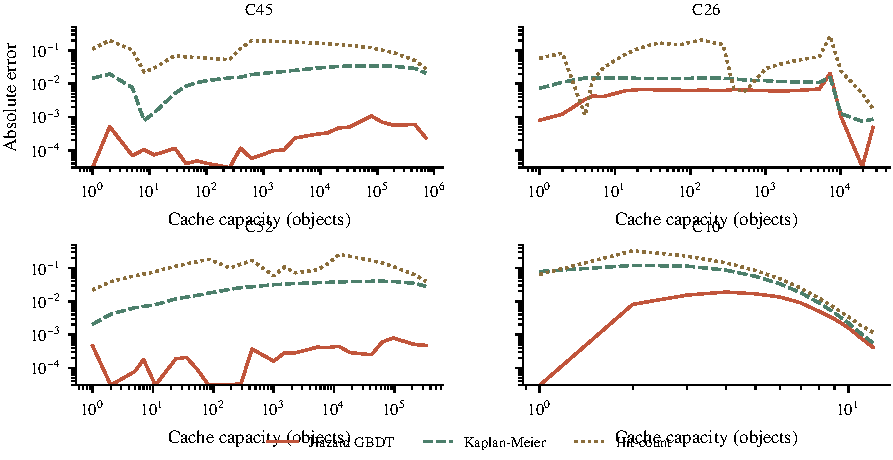
\includegraphics[width=\linewidth]{figures/cluster-error.pdf}
\captionof{figure}{Absolute curve error against capacity, log-log, one panel per
trace. Hazard GBDT solid, Kaplan-Meier dashed, hit-count dotted. Exact zeros are
floored at $3\times10^{-5}$, below every measured hazard error.}
\label{fig:cluster-error}
\end{minipage}
\end{center}

\subsection{Capacity ratio figure}
\label{app:capacity-figure}

\begin{center}
\begin{minipage}{0.62\linewidth}
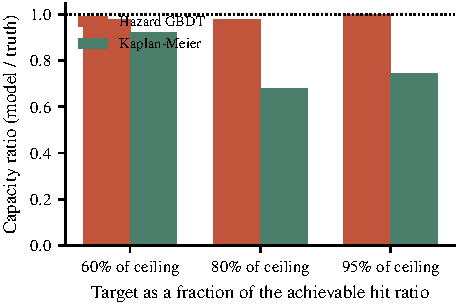
\includegraphics[width=\linewidth]{figures/capacity-ratio.pdf}
\captionof{figure}{Capacity ratio at three targets, median over the four traces,
with parity dotted. Below one is under-provisioning.}
\label{fig:capacity-ratio}
\end{minipage}
\end{center}

\subsection{Trace design numbers}
\label{app:traces}

\begin{table}[h]
\centering
\footnotesize
\sisetup{group-separator={,},group-minimum-digits=4}
\caption{The four traces, first 5{,}000{,}000 requests each. Eligible is the
fraction with a previous access inside the window; $p_c$ is its complement and is
the compulsory mass. $R$ is the backward reuse distance in objects. Bins and grid
points are realised counts; $b_{M-1}$ is the lower edge of the overflow bin, and
every reported capacity is below it.}
\label{tab:traces}
\begin{tabular}{@{}l r r r r r r r r@{}}
\toprule
Trace & {Keys} & {Mean object (B)} & {Eligible} & {$p_c$} & {$R$ p50} & {$R$ p99} & {Bins / grid} \\
\midrule
cluster45 & \num{2158200} & \num{91} & 0.568 & 0.432 & \num{4} & \num{1008186} & 33 / 24 \\
cluster26 & \num{394747} & \num{1046} & 0.921 & 0.079 & \num{472} & \num{17709} & 33 / 24 \\
cluster52 & \num{932119} & \num{252} & 0.814 & 0.186 & \num{1097} & \num{488644} & 33 / 24 \\
cluster10 & \num{2500051} & \num{1289} & 0.500 & 0.500 & \num{1} & \num{8} & 14 / 12 \\
\bottomrule
\end{tabular}
\end{table}


\end{document}
